\documentclass[letterpaper]{article}

\usepackage{hyperref}
\usepackage{tikz}

\title{Amazon Delivery Truck Simulation}
\author{Hanna Butt \thanks{HFB352} \and Ashton Cole \thanks{AVC687, \href{mailto:ashtonc24@utexas.edu}{ashtonc24@utexas.edu}} \and Kelechi Emeruwa \thanks{KEE688}}
\date{\today}

\begin{document}
    \maketitle

    \begin{abstract}
        Summary of whole paper.
    \end{abstract}

    \section{Introduction}
    Introduce the context and the problem here.

    \section{Methodology}
    Talk about how we're solving the problem (C++, TACC super computer) and how the program works (e.g. reads in text file, spits out text file). Then go into the development process (start simple with address/list classes, test functionality then expand it a bit)

    \section{Results}
    Pretty pictures go here. Describe each situation being displayed and talk about what they mean, e.g. is it the optimal solution? Good enough? Is there a tradeoff between time to execute and quality of results?

    Hmm, maybe insert a table comparing number of nodes/trucks to program execution time. What rate does it increase at $(O(n), O(n^2), \&c.)$

    \subsection{Simple Single-Truck Case}


    %%%%%%
    %%%%%% MOVE THIS SOMEWHERE USEFUL
    %%%%%%
    \begin{figure}[h]
        \caption{An unsorted route optimized through the greedy method (blue) and the opt2 method(green). This demonstrates how the opt2 method alone is not necessarily sufficient to find the fastest route.}
        \begin{minipage}{0.3\linewidth}
            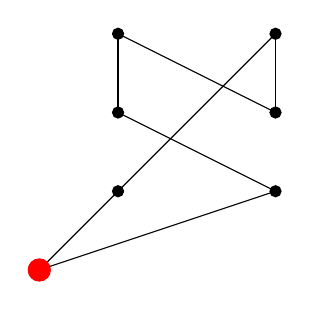
\begin{tikzpicture}
                % Old
                \draw [black] (0, 0) -- (1, 1);
                \filldraw [black] (0, 0) circle (2pt);
                \draw [black] (1, 1) --(3, 3);
                \filldraw [black] (1, 1) circle (2pt);
                \draw [black] (3, 3) --(3, 2);
                \filldraw [black] (3, 3) circle (2pt);
                \draw [black] (3, 2) --(1, 3);
                \filldraw [black] (3, 2) circle (2pt);
                \draw [black] (1, 3) --(1, 2);
                \filldraw [black] (1, 3) circle (2pt);
                \draw [black] (1, 2) --(3, 1);
                \filldraw [black] (1, 2) circle (2pt);
                \draw [black] (3, 1) --(0, 0);
                \filldraw (3, 1) [black] circle (2pt);
                \filldraw [red] (0, 0) circle (4pt);
            \end{tikzpicture}
        \end{minipage}
        \begin{minipage}{0.3\linewidth}
            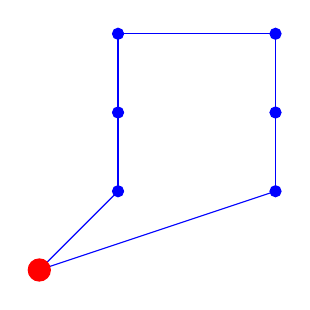
\begin{tikzpicture}
                % Greedy
                \draw [blue] (0, 0) -- (1, 1);
                \filldraw [blue] (0, 0) circle (2pt);
                \draw [blue] (1, 1) --(1, 2);
                \filldraw [blue] (1, 1) circle (2pt);
                \draw [blue] (1, 2) --(1, 3);
                \filldraw [blue] (1, 2) circle (2pt);
                \draw [blue] (1, 3) --(3, 3);
                \filldraw [blue] (1, 3) circle (2pt);
                \draw [blue] (3, 3) --(3, 2);
                \filldraw [blue] (3, 3) circle (2pt);
                \draw [blue] (3, 2) --(3, 1);
                \filldraw [blue] (3, 2) circle (2pt);
                \draw [blue] (3, 1) --(0, 0);
                \filldraw (3, 1) [blue] circle (2pt);
                \filldraw [red] (0, 0) circle (4pt);
            \end{tikzpicture}
        \end{minipage}
        \begin{minipage}{0.3\linewidth}
            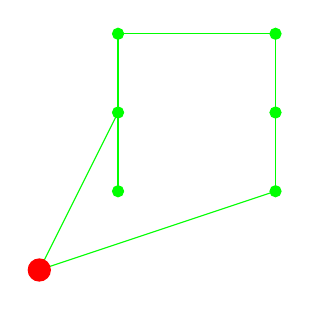
\begin{tikzpicture}
                % opt2
                \draw [green] (0, 0) -- (1, 2);
                \filldraw [green] (0, 0) circle (2pt);
                \draw [green] (1, 2) --(1, 1);
                \filldraw [green] (1, 2) circle (2pt);
                \draw [green] (1, 1) --(1, 3);
                \filldraw [green] (1, 1) circle (2pt);
                \draw [green] (1, 3) --(3, 3);
                \filldraw [green] (1, 3) circle (2pt);
                \draw [green] (3, 3) --(3, 2);
                \filldraw [green] (3, 3) circle (2pt);
                \draw [green] (3, 2) --(3, 1);
                \filldraw [green] (3, 2) circle (2pt);
                \draw [green] (3, 1) --(0, 0);
                \filldraw (3, 1) [green] circle (2pt);
                \filldraw [red] (0, 0) circle (4pt);
            \end{tikzpicture}
        \end{minipage}
    \end{figure}

    \subsection{Difficult Single-Truck Case}

    \section{Conclusion}
    Talk about what we learned, how this all applies to industry, ideas to scale the problem up, \&c.
\end{document}